% Created 2021-07-20 ter 18:04
% Intended LaTeX compiler: pdflatex
\documentclass[aspectratio=169,presentation,mathserif,10pt]{beamer}
\usepackage[utf8]{inputenc}
\usepackage[T1]{fontenc}
\usepackage{graphicx}
\usepackage{grffile}
\usepackage{longtable}
\usepackage{wrapfig}
\usepackage{rotating}
\usepackage[normalem]{ulem}
\usepackage{amsmath}
\usepackage{textcomp}
\usepackage{amssymb}
\usepackage{capt-of}
\usepackage{hyperref}
\usepackage[brazil, portuguese]{babel} \usepackage{icomma} \usepackage{helvet} \setbeamerfont{caption}{size=\tiny}
\mode<beamer>{\usetheme{Antibes}\usecolortheme{beaver}\institute[DTECH-UFSJ]{DTECH-UFSJ}}
\AtBeginSection[]{\begin{frame}<beamer>\frametitle{Tópicos}\tableofcontents[currentsection]\end{frame}}
\usetheme{default}
\author{João Pedro Hallack Sansão}
\date{Julho/2021}
\title{Conceitos iniciais sobre aprendizado de máquina}
\hypersetup{
 pdfauthor={João Pedro Hallack Sansão},
 pdftitle={Conceitos iniciais sobre aprendizado de máquina},
 pdfkeywords={},
 pdfsubject={},
 pdfcreator={Emacs 26.1 (Org mode 9.1.9)}, 
 pdflang={Portuguese}}
\begin{document}

\maketitle
\begin{frame}{Outline}
\tableofcontents
\end{frame}








\section{Aprendizado de máquina}
\label{sec:org739c244}

\begin{frame}[label={sec:org9621850}]{Aprendizado de máquina (Machine Learning)}
\begin{itemize}
\item Definição clássica: "Campo de estudo que dá aos computadores a
habilidade de aprender sem ser explicitamente programados."

\item Definição moderna: "Um programa de computador aprende com a
experiência E no que diz respeito a alguma classe de tarefas T e
medida de desempenho P, se o seu desempenho nas tarefas em T,
conforme medido por P, melhora com a experiência E."
\end{itemize}
\end{frame}



\begin{frame}[label={sec:orgc98bbc7}]{Aprendizado de máquina x Programação tradicional}
\begin{figure}[htbp]
\centering
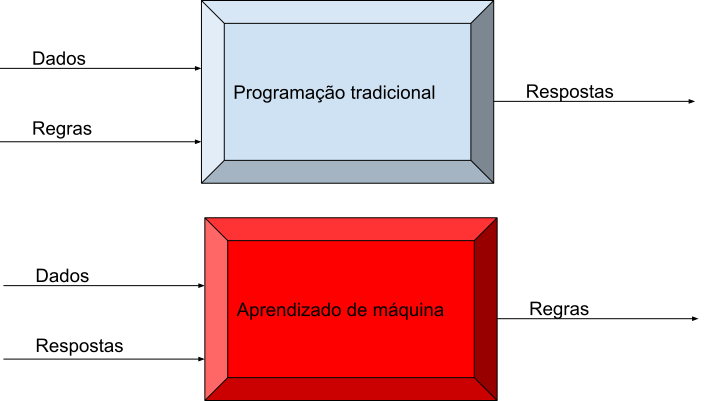
\includegraphics[height=0.7\textheight]{./fig/mlct.png}
\caption{Adaptado de Moroney (2020)}
\end{figure}
\end{frame}


\begin{frame}[label={sec:org1e3885d}]{Exemplos:}
\begin{columns}
\begin{column}{0.5\columnwidth}
\begin{figure}[htbp]
\centering
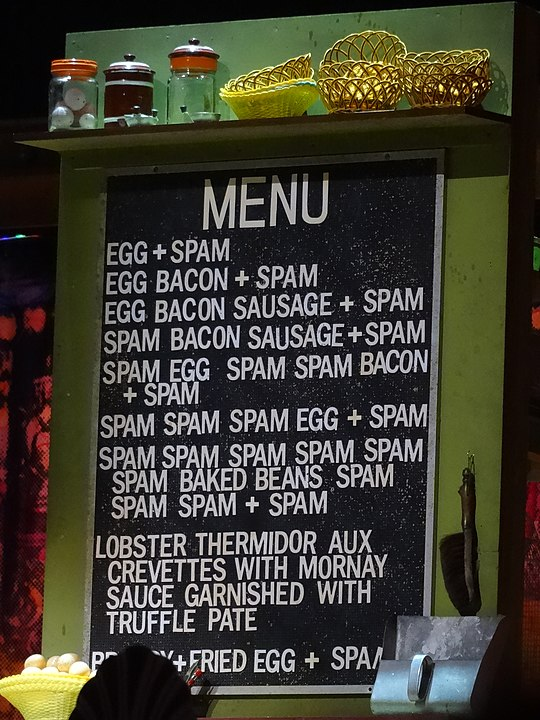
\includegraphics[height=.7\textheight]{./fig/spam.jpg}
\caption{\url{https://youtu.be/_bW4vEo1F4E}}
\end{figure}
\end{column}



\begin{column}{0.5\columnwidth}
\begin{itemize}
\item Filtragem de SPAM 

\begin{itemize}
\item Tarefa (T): classificação de e-mails como SPAM ou não
\item Experiência (E): observação de rotulação dos e-mails como SPAM ou não
\item Desempenho (P): Fração dos emails corretamente classificados
\end{itemize}
\end{itemize}
\end{column}
\end{columns}
\end{frame}



\begin{frame}[label={sec:org7e32bd3}]{Exemplos (continuação):}
\begin{columns}
\begin{column}{0.5\columnwidth}
\begin{figure}[htbp]
\centering
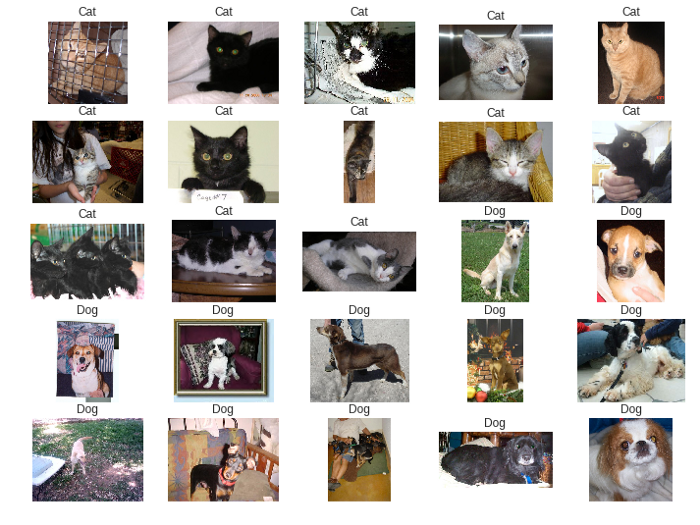
\includegraphics[height=.7\textheight]{./fig/catxdog.png}
\caption{\url{https://medium.com/abraia/first-steps-with-transfer-learning-for-custom-image-classification-with-keras-b941601fcad5}}
\end{figure}
\end{column}

\begin{column}{0.5\columnwidth}
\begin{itemize}
\item Gato x Cão
\begin{itemize}
\item Tarefa (T): classificação como gato ou cão
\item Experiência (E): rotulação da imagem como gato (0) ou cão (1)
\item Desempenho (P): Fração das imagens corretamente classificadas
\end{itemize}
\end{itemize}
\end{column}
\end{columns}
\end{frame}



\begin{frame}[label={sec:org4df46a8}]{Classificação de algoritmos de Aprendizado de máquina}
\begin{itemize}
\item Aprendizado supervisionado
\item Aprendizado não-supervisionado
\item Aprendizado por reforço
\end{itemize}
\end{frame}


\begin{frame}[label={sec:org07d1567}]{Aprendizado supervisionado x não supervisionado}
\begin{figure}[htbp]
\centering
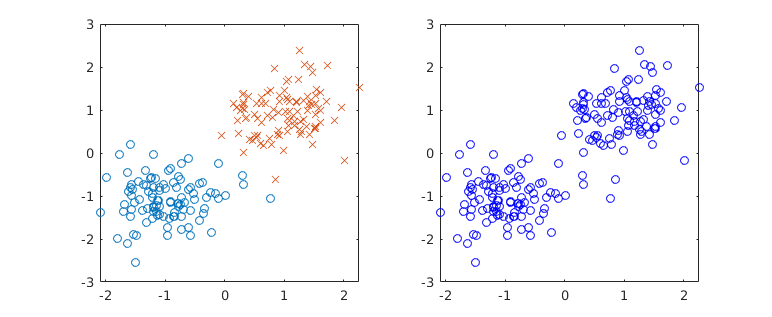
\includegraphics[height=0.6\textheight]{./fig/sxns.png}
\caption{Elaboração própria}
\end{figure}
\end{frame}
\end{document}